\UC{Registrazione}
\begin{figure}[H]
	\centering
	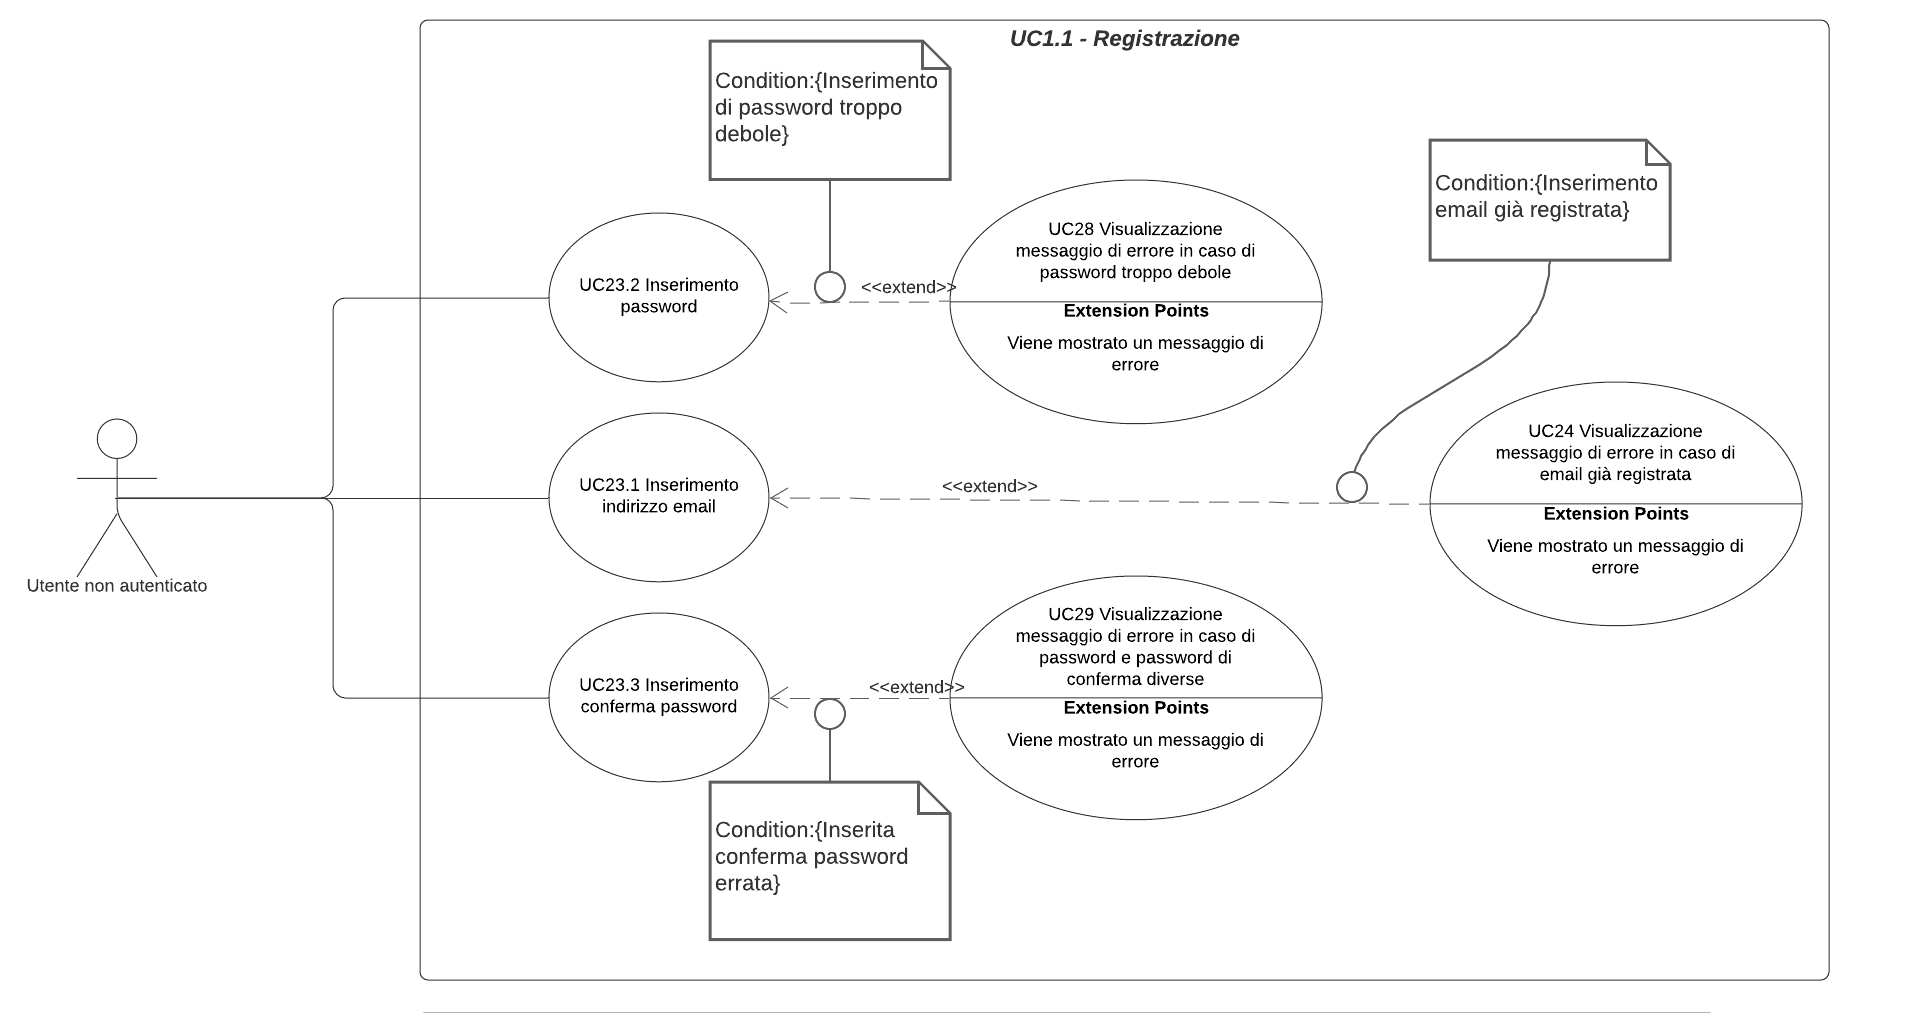
\includegraphics[scale=0.6]{Immagini/DiagrammiUC/UC1.1Registrazione}
	\caption{Diagramma di \actualUC: Registrazione}
	\label{fig:RegistrazionePiattaforma}
\end{figure}

L'utente non autenticato che non dispone di credenziali può registrarsi e accedere come acquirente nella piattaforma compilando alcuni campi obbligatori per poter procedere.
\begin{itemize}
	\item \textbf{Attori primari:} utente non autenticato;
	\item \textbf{Attori secondari:} \glo{identity manager};
	\item \textbf{Precondizione:} l'utente non è ancora presente nella piattaforma;
	\item \textbf{Postcondizione:} l'utente è registrato con un account acquirente ed è autenticato come tale sulla piattaforma;
	\item \textbf{Scenario principale:}
	\begin{itemize}
		\item L'utente accede al sistema;
		\item L'utente non autenticato si trova nella schermata di registrazione;
		\item (UC) - Inserisce tutti i dati per compilare il modulo di registrazione;
		\item L'utente non autenticato conferma il proprio indirizzo email inserito;
		\item L'utente possiede un account presso il sistema.
	\end{itemize}
	\item \textbf{Estensioni:}
	\begin{enumerate}[label=\lett]
		\item L'utente inserisce un indirizzo email e l'identity manager segnala che è già presente nella piattaforma
		\begin{itemize}
			\item L'utente non viene registrato presso il sistema;
			\item (UC) - Visualizzazione messaggio di errore in caso di email già registrata nella piattaforma;
			\item Viene fornita all'utente la possibilità di modificare il proprio indirizzo email inserito.
		\end{itemize}
		\item L'utente compila i campi dati per la password e la conferma della stessa con due password diverse, in questo caso:
		\begin{itemize}
			\item L'utente non viene registrato presso il sistema;
			\item L'identity manager segnala che le due password inserite non coincidono;
			\item (UC) - Visualizzazione messaggio di errore in caso di password e password di conferma diverse;
			\item L'utente può modificare le password inserite.
		\end{itemize}
	\end{enumerate}
\end{itemize}

\subUC{Inserimento dati per la registrazione}
L'utente compila il modulo per proseguire con la registrazione presso la piattaforma.
\begin{itemize}
	\item \textbf{Attori primari:} utente non autenticato;
	\item \textbf{Attori secondari:} identity manager;
	\item \textbf{Precondizione:} l'utente non è autenticato e si trova all'interno della schermata di registrazione;
	\item \textbf{Postcondizione:} l'utente ha compilato il modulo e può procedere con la registrazione;
	\item \textbf{Scenario principale:} l'utente non autenticato compila i campi nel seguente modo:
	\begin{itemize}
		\item (UC) - Inserimento nome per la registrazione;
		\item (UC) - Inserimento cognome per la registrazione;
		\item (UC) - Inserimento indirizzo e-mail per la registrazione;
		\item (UC) - Inserimento password per la registrazione;
		\item (UC) - Inserimento conferma password.
	\end{itemize}
\end{itemize}

\subUC{Inserimento del nome per la registrazione}
\begin{itemize}
	\item \textbf{Attori primari:} utente non autenticato;
	\item \textbf{Attori secondari:} identity manager;
	\item \textbf{Precondizione:} l'utente non è autenticato;
	\item \textbf{Postcondizione:} l'utente ha inserito il proprio nome;
	\item \textbf{Scenario principale:} l'utente non autenticato inserisce il proprio nome per la registrazione;
	\item \textbf{Estensioni:}
	\begin{enumerate}[label=\lett]
		\item L'utente non inserisce il nome e l'identity manager controlla il campo dati per il nome che non risulta compilato, in questo caso:
		\begin{itemize}
			\item (UC) - Viene mostrato un messaggio d'errore campo dati obbligatorio non inserito;
			\item Viene fornita all'utente la possibilità di inserire un nome.
		\end{itemize}
	\end{enumerate} 
\end{itemize}

\subUC{Inserimento del cognome per la registrazione}
\begin{itemize}
	\item \textbf{Attori primari:} utente non autenticato;
	\item \textbf{Attori secondari:} identity manager;
	\item \textbf{Precondizione:} l'utente non è autenticato;
	\item \textbf{Postcondizione:} l'utente ha inserito il proprio cognome;
	\item \textbf{Scenario principale:} l'utente non autenticato inserisce il proprio cognome per la registrazione;
	\item \textbf{Estensioni:}
	\begin{enumerate}[label=\lett]
		\item L'utente non inserisce il cognome e l'identity manager controlla il campo dati per il cognome che non risulta compilato, in questo caso:
		\begin{itemize}
			\item (UC) - Viene mostrato un messaggio d'errore campo dati obbligatorio non inserito;
			\item Viene fornita all'utente la possibilità di inserire un cognome.
		\end{itemize}
	\end{enumerate}
\end{itemize}

\subUC{Inserimento indirizzo email per la registrazione}
L'utente non autenticato inserisce l'indirizzo email.
\begin{itemize}
	\item \textbf{Attori primari:} utente non autenticato;
	\item \textbf{Attori secondari:} identity manager;
	\item \textbf{Precondizione:} l'utente non autenticato non ha ancora fornito un'email ed ha a disposizione un campo dati dove inserirla;
	\item \textbf{Postcondizione:} l'utente non autenticato ha fornito un indirizzo email valido;
	\item \textbf{Scenario principale:} l'utente non autenticato inserisce il proprio indirizzo email per procedere con la registrazione;
	\item \textbf{Estensioni:}
	\begin{enumerate}[label=\lett]
		\item L'utente non inserisce l'email e l'identity manager controlla il campo dati che risulta essere vuoto, in questo caso:
		\begin{itemize}
			\item (UC) - Viene mostrato un messaggio d'errore campo dati obbligatorio non inserito;
			\item Viene fornita all'utente la possibilità di inserire un indirizzo email.
		\end{itemize}
		\item L'utente non autenticato ha inserito un indirizzo email e l'identity manager segnala che non è nel formato non corretto, in questo caso:
		\begin{itemize}
			\item (UC) - Viene mostrato un messaggio d'errore indirizzo email non rispetta il formato;
			\item Viene fornita all'utente la possibilità di modificare l'indirizzo email inserito.
		\end{itemize}
	\end{enumerate}
\end{itemize}

\subUC{Inserimento password per la registrazione}
L'utente non autenticato inserisce una password.
\begin{itemize}
	\item \textbf{Attori primari:} utente non autenticato;
	\item \textbf{Attori secondari:} identity manager;
	\item \textbf{Precondizione:} l'utente non autenticato non ha ancora fornito una password che rispetta i requisiti di complessità ed ha a disposizione un campo dati dove inserirla;
	\item \textbf{Postcondizione:} l'utente ha inserito una password valida;
	\item \textbf{Scenario principale:} l'utente non autenticato inserisce una password che rispetti le condizioni imposte per procedere con la registrazione;
	\item \textbf{Estensioni:}
	\begin{enumerate}[label=\lett]
		\item L'utente non inserisce la password e l'identity manager controlla il campo dati che risulta essere vuoto, in questo caso:
		\begin{itemize}
			\item (UC) - Viene mostrato un messaggio d'errore campo dati obbligatorio non inserito;
			\item Viene fornita all'utente la possibilità di inserire una password.
		\end{itemize}
		\item L'utente non autenticato ha inserito una password e l'identity manager segnala che non è nel formato corretto, in questo caso:
		\begin{itemize}
			\item (UC) - Viene mostrato un messaggio d'errore password non rispetta i requisiti di complessità;
			\item Viene fornita all'utente la possibilità di modificare la password inserita.
		\end{itemize}
	\end{enumerate} 
\end{itemize}

\subUC{Inserimento conferma password per la registrazione}
L'utente non autenticato inserisce una password.
\begin{itemize}
	\item \textbf{Attori primari:} utente non autenticato;
	\item \textbf{Attori secondari:} identity manager;
	\item \textbf{Precondizione:} l'utente non autenticato non ha ancora fornito una password che rispetta i requisiti di complessità ed ha a disposizione un campo dati dove inserirla;
	\item \textbf{Postcondizione:} l'utente ha inserito la conferma della password ed è valida.
	\item \textbf{Scenario principale:} l'utente non autenticato inserisce una password che rispetti le condizioni imposte per procedere con la registrazione;
	\item \textbf{Estensioni:} 
	\begin{enumerate}[label=\lett]
		\item L'utente non inserisce la conferma password e l'identity manager controlla il campo dati che risulta essere vuoto, in questo caso:
		\begin{itemize}
			\item (UC) - Viene mostrato un messaggio d'errore campo dati obbligatorio non inserito;
			\item Viene fornita all'utente la possibilità di inserire una password.
		\end{itemize}
		\item L'utente non autenticato ha inserito una password e l'identity manager segnala che non è nel formato corretto, in questo caso:
		\begin{itemize}
			\item (UC) - Viene mostrato un messaggio d'errore password non rispetta i requisiti di complessità;
			\item Viene fornita all'utente la possibilità di modificare la password inserita.
		\end{itemize}
	\end{enumerate} 
\end{itemize}

\UC{Autenticazione nella piattaforma con credenziali venditore}
\begin{figure}[H]
    \centering
    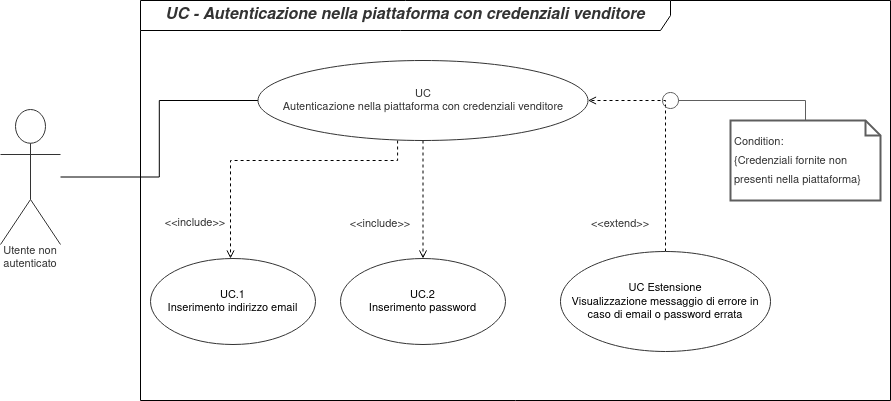
\includegraphics[scale=0.6]{Immagini/DiagrammiUC/AccessoVenditore.png}
    \caption{Diagramma di \actualUC: Autenticazione nella piattaforma con credenziali venditore} 
    \label{fig:LoginVenditore}
\end{figure}

L'utente non autenticato che dispone di credenziali venditore può accedere nella piattaforma usando l'email e la password.
\begin{itemize}
    \item \textbf{Attori primari:} utente non autenticato;
    \item \textbf{Attori secondari:} identity manager;
    \item \textbf{Precondizione:} l'utente dispone di credenziali venditore;
    \item \textbf{Postcondizione:} l'utente è autenticato come venditore e si trova sulla \glo{dashboard};
    \item \textbf{Scenario principale:}
    \begin{itemize}
    	\item L'utente accede al sistema;
    	\item L'utente non autenticato si trova nella schermata di login;
    	\item (UC) - Inserisce tutti i dati per compilare il modulo di autenticazione; %Inserisce le credenziali per accedere alla piattaforma
    	\item L'utente richiede l'autenticazione;
    	\item L'utente è autenticato come venditore all'interno della piattaforma;
    	\item L'utente viene portato alla dashboard.
    \end{itemize}
	\item \textbf{Estensioni:}
	\begin{enumerate}[label=\lett]
		\item L'utente compila i campi dati con delle credenziali, richiede l'autenticazione e l'identity manager segnala che le credenziali fornite non appartengono alla piattaforma
		\begin{itemize}
			\item L'utente non viene autenticato presso il sistema;
			\item (UC) - Viene visualizzato un messaggio di errore credenziali non presenti nella piattaforma;
			\item Viene fornita all'utente la possibilità di modificare i valori inseriti nel modulo di autenticazione.
		\end{itemize}
	\end{enumerate} 
\end{itemize}

\resetSubUC
\subUC{Inserimento dati per l'autenticazione}
L'utente compila il modulo per proseguire con l'autenticazione presso la piattaforma.
\begin{itemize}
	\item \textbf{Attori primari:} utente non autenticato;
	\item \textbf{Attori secondari:} identity manager;
	\item \textbf{Precondizione:} l'utente non è autenticato e si trova all'interno della schermata di login;
	\item \textbf{Postcondizione:} l'utente ha compilato il modulo e può procedere con l'autenticazione;
	\item \textbf{Scenario principale:} l'utente non autenticato compila i campi nel seguente modo:
	\begin{itemize}
		\item (UC) - Inserimento indirizzo e-mail per l'autenticazione;
		\item (UC) - Inserimento password per l'autenticazione.
	\end{itemize}
\end{itemize}

\subUC{Inserimento indirizzo email per l'autenticazione}
L'utente non autenticato inserisce l'indirizzo email.
\begin{itemize}
	\item \textbf{Attori primari:} utente non autenticato;
	\item \textbf{Attori secondari:} identity manager;
	\item \textbf{Precondizione:} l'utente non autenticato possiede delle credenziali d'accesso e si trova nella schermata di login;
	\item \textbf{Postcondizione:}  l'utente ha inserito il proprio indirizzo email;
	\item \textbf{Scenario principale:} l'utente non autenticato inserisce il proprio indirizzo email per procedere con l'autenticazione;
	\item \textbf{Estensioni:}
	\begin{enumerate}[label=\lett]
		\item L'utente non inserisce l'email e l'identity manager controlla il campo dati che risulta essere vuoto, in questo caso:
		\begin{itemize}
			\item (UC) - Viene mostrato un messaggio d'errore campo dati obbligatorio non inserito;
			\item Viene fornita all'utente la possibilità di inserire un indirizzo email.
		\end{itemize}
	\end{enumerate}
\end{itemize}

\subUC{Inserimento password per l'autenticazione}
L'utente non autenticato inserisce una password.
\begin{itemize}
	\item \textbf{Attori primari:} utente non autenticato;
	\item \textbf{Attori secondari:} identity manager;
	\item \textbf{Precondizione:} l'utente non autenticato possiede delle credenziali d'accesso e si trova nella schermata di login;
	\item \textbf{Postcondizione:} l'utente ha inserito la propria password;
	\item \textbf{Scenario principale:} l'utente non autenticato inserisce la propria password per procedere con l'autenticazione;
	\item \textbf{Estensioni:} 
	\begin{enumerate}[label=(\alph*)]
		\item L'utente non inserisce la password e l'identity manager controlla il campo dati che risulta essere vuoto, in questo caso:
		\begin{itemize}
			\item (UC) - Viene mostrato un messaggio d'errore campo dati obbligatorio non inserito;
			\item Viene fornita all'utente la possibilità di inserire una password.
		\end{itemize}
	\end{enumerate} 
\end{itemize}

\UC{Autenticazione nella piattaforma con credenziali acquirente}
\begin{figure}[H]
	\centering
	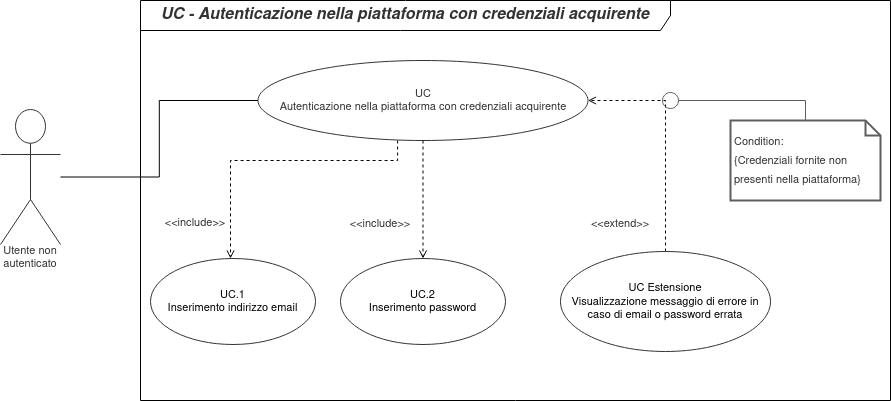
\includegraphics[scale=0.6]{Immagini/DiagrammiUC/AccessoAcquirente.png}
	\caption{Diagramma di \actualUC: Autenticazione nella piattaforma con credenziali acquirente} 
	\label{fig:LoginAcquirente}
\end{figure}

L'utente non autenticato che dispone di credenziali acquirente può accedere nella piattaforma usando l'email e la password.
\begin{itemize}
	\item \textbf{Attori primari:} utente non autenticato;
	\item \textbf{Attori secondari:} identity manager;
	\item \textbf{Precondizione:} l'utente dispone di credenziali acquirente;
	\item \textbf{Postcondizione:} l'utente è autenticato come acquirente e si trova nella schermata principale;
	\item \textbf{Scenario principale:}
	\begin{itemize}
		\item L'utente accede al sistema;
		\item L'utente non autenticato si trova nella schermata di login;
		\item (UC) - Inserisce tutti i dati per compilare il modulo di autenticazione; %Inserisce le credenziali per accedere alla piattaforma
		\item L'utente richiede l'autenticazione;
		\item L'utente è autenticato come acquirente all'interno del sistema;
		\item L'utente viene portato alla schermata principale della piattaforma.
	\end{itemize}
	\item \textbf{Estensioni:}
	\begin{enumerate}[label=\lett]
		\item L'utente compila i campi dati con delle credenziali, richiede l'autenticazione e l'identity manager segnala che le credenziali fornite non appartengono alla piattaforma
		\begin{itemize}
			\item L'utente non viene autenticato presso il sistema;
			\item (UC) - Viene visualizzato un messaggio di errore credenziali non presenti nella piattaforma;
			\item Viene fornita all'utente la possibilità di modificare i valori inseriti nel modulo di autenticazione.
		\end{itemize}
	\end{enumerate} 
\end{itemize}

%Inserimento dati per l'autenticazione, inserimento indirizzo email per l'autenticazione e inserimento password per l'autenticazione sono in comune

\UC{Password dimenticata}
\begin{figure}[H]
    \centering
    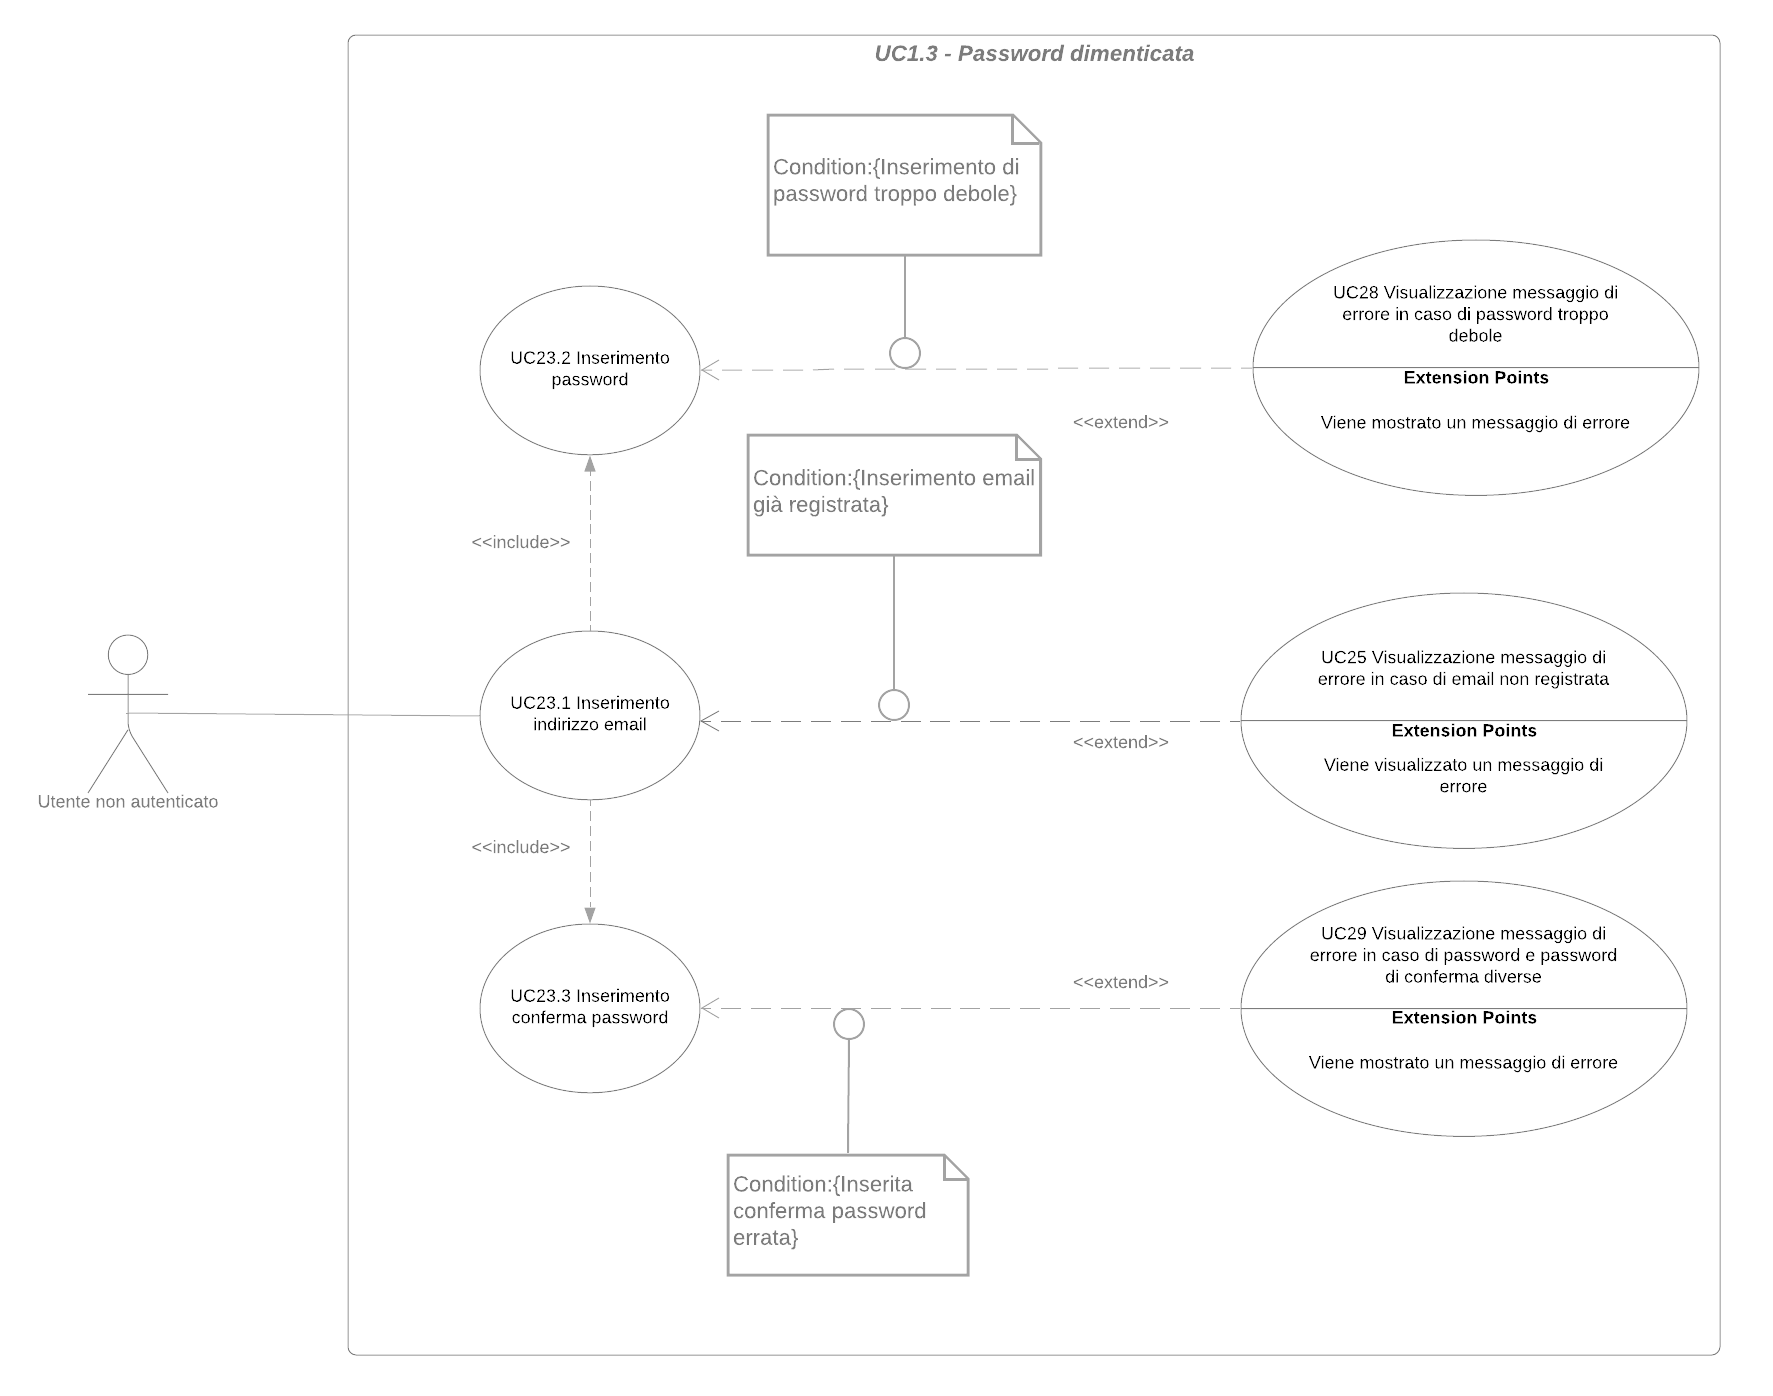
\includegraphics[scale=0.2]{Immagini/DiagrammiUC/UC1.3PasswordDimenticata.png}
    \caption{Diagramma di \actualUC: Password dimenticata} 
    \label{fig:PasswordDimenticata}
\end{figure}

L'utente che dispone di credenziali si è dimenticato la propria password e la vuole cambiare.
\begin{itemize}
    \item \textbf{Attori primari:} utente non autenticato;
    \item \textbf{Autori secondari:} identity manager;
    \item \textbf{Precondizione:} l'utente non autenticato che dispone di credenziali si trova nella schermata per cambiare la password;
    \item \textbf{Postcondizione:} l'utente è autenticato e ha cambiato la password con cui poter effettuare l'accesso alla piattaforma;
    \item \textbf{Scenario principale:} l'utente che dispone di credenziali si è dimenticato la propria password e per cambiarla deve compiere i seguenti passi:
    \begin{itemize}
        \item (UC) - Inserimento indirizzo email;
        \item Invio link per il cambio della password all'indirizzo email indicato;
        \item Apertura della schermata per il cambio della password;
        \item (UC) - Inserimento nuova password;
        \item (UC) - Inserimento conferma nuova password;
        \item L'utente è autenticato e ha cambiato la password.
    \end{itemize}
	\item \textbf{Estensioni:}
	\begin{enumerate}[label=\lett]
		\item L'utente inserisce un indirizzo email e l'identity manager segnala che l'indirizzo email non è presente nella piattaforma
		\begin{itemize}
			\item (UC) - Viene visualizzato un messaggio di errore indirizzo email non registrato nella piattaforma;
			\item L'utente rimane non autenticato e alla schermata per cambiare la password.
		\end{itemize}
		\item L'utente compila i campi dati
		\begin{itemize}
			\item (UC) - Inserimento indirizzo email;
			\item Invio link per il cambio della password all'indirizzo email indicato;
			\item Apertura della schermata per il cambio della password;
			\item (UC) - Inserimento nuova password;
			\item (UC) - Inserimento conferma nuova password.
		\end{itemize}
		Ma l'identity manager segnala che le due password inserite non coincidono
		\begin{itemize}
			\item (UC) - Visualizzazione messaggio di errore in caso di password e password di conferma diverse.
			\item L'utente può modificare le password inserite.
		\end{itemize}
	\end{enumerate}
\end{itemize}

\UC{Logout dalla piattaforma}
L'utente autenticato decide di scollegarsi dalla piattaforma.
\begin{itemize}
    \item \textbf{Attori primari:} utente autenticato;
    \item \textbf{Precondizione:} l'utente ha eseguito il login precedentemente e vuole scollegarsi dalla piattaforma;
    \item \textbf{Postcondizione:} l'utente autenticato diventa un utente non autenticato;
    \item \textbf{Scenario principale:} l'utente autenticato decide di scollegarsi dalla piattaforma e compie l'azione di scollegamento.
\end{itemize}